\documentclass[colorinlistoftodos]{article}
\usepackage[utf8]{inputenc}
\usepackage{natbib}
\usepackage{usebib}
\bibinput{bibliography}
\usepackage[spanish]{babel}
\usepackage[numbib,nottoc]{tocbibind}
\usepackage[table]{xcolor}
\usepackage{makecell}
\usepackage{graphicx}
\usepackage{adjustbox}
\usepackage{amsmath}
\usepackage{amssymb}
\usepackage[font=footnotesize]{caption}
\usepackage{longtable}
\usepackage[hidelinks]{hyperref}
\usepackage{todonotes}
\setcounter{tocdepth}{2}
\renewcommand\spanishtablename{Tabla}

\definecolor{highlight-blue}{rgb}{
    0.12156862745098039, 0.4666666666666667, 0.7058823529411765
}
\definecolor{highlight-orange}{rgb}{
    1.0, 0.4980392156862745, 0.054901960784313725
}

\hypersetup{
    colorlinks=true,
    urlcolor=blue,
    linkcolor=blue,
    filecolor=black,
    linkcolor=black,
    citecolor=black
}


\title{
    {\large Universidad de Buenos Aires\vspace{20pt}}\\
    {
\includegraphics[scale=0.4]{images/uba.eps}}\\
    {\large\textbf{Facultad de Ciencias Exactas y Naturales}}\vspace{16pt}\\
    {\small\textbf{Especializaci\'on en Exploraci\'on de Datos\\y Descubrimiento del Conocimiento}\vspace{16pt}}\\
    {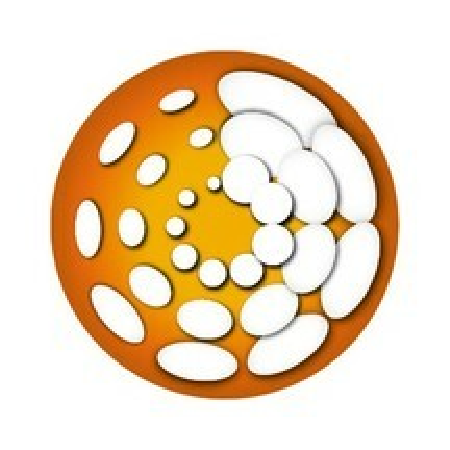
\includegraphics[scale=0.5]{images/master.eps}}\\
    {
        Selecci\'on de técnicas estadísticos\\
        para la vectorización de discursos políticos\\
        referidos a la reglamentaci\'on del acceso al aborto
    }
}
\author{Autora:\\Fern\'andez Urquiza, Macarena}
\date{Fecha: 30 -- 09 -- 2024}

\begin{document}
\clearpage\maketitle
\thispagestyle{empty}

\newpage
\tableofcontents

\newpage

\begin{abstract}
En este trabajo se aborda la selección y evaluación de rasgos para el
entrenamiento de modelos de aprendizaje automatizado aplicado sobre datos textuales.
El \textit{corpus} con el que se trabajó pertenece a la transcripción taquigráfica
de la sesión del Senado de la Nación Argentina para la reglamentación del acceso
al aborto, la cual fue obtenida mediante la técnica de \textit{scraping}. Durante el
procesamiento de los datos se recurrió a una lematización automatizada sobre la que
luego se realizó una corrección manual. Los datos fueron vectorizados empleando
métodos estadísticos tomados de \cite{monroe2008fightin}, que permitieron la selección
de rasgos y el posterior entrenamiento de un modelo de Regresión Logísitca.
\end{abstract}

\section{Introducci\'on}\label{section-intro}

\subsection{Antecedentes}\label{subsection-intro-background}
El ``Encuentro nacional de mujeres'' consiste en un evento de alcance nacional
en el territorio argentino que se realiza de manera anual desde 1986 y se propone
auto-convocado, democr\'atico, pluralista y federal.
Como fruto de este evento surge, en 2005, la ``Campaña nacional por el derecho al
aborto legal, seguro y gratuito'', una alianza de organizaciones que promueve y
lucha por la educaci\'on sexual como pilar fundamental en la decisi\'on sobre la gestaci\'on,
el acceso a m\'etodos anticonceptions que permitan la adecuada prevenci\'on de embarazos
no deseados, y el aborto legal, seguro y grauito que le posibilite a la persona gestante
discontinuar con un embarazo si no desea atravesarlo.
Hacia 2007, la Campaña redacta y presenta el ``Proyecto de ley de interrupci\'on
voluntaria del embarazo'' como iniciativa social para que sea considerado por los
legisladores y, as\'i, llegue a ser tratado en el Congreso de la Naci\'on.
Pero no es sino hasta junio de 2018, y luego de reiteradas presentaciones, que logran
contar con el aval de entre 20 y 70 diputados. Reci\'en entonces el proyecto llega a
ser debatido en la C\'amara de dichos legisladores, donde logra media sanci\'on.
Posteriormente, la C\'amara de Senadores lo rechaza.
En diciembre de 2020, el proyecto se vuelve a tratar y, esta vez, logra la aprobaci\'on
del Congreso.
La ley 27.610, sobre el ``Acceso a la interrupci\'on voluntaria del embarazo'', entr\'o
en vigencia en la Argentina el 24 de enero de 2021 y regula el acceso a la
interrupci\'on voluntaria del embarazo y a los cuidados postaborto para todas
las personas con capacidad de gestar.\footnote{\cite{campana@lalucha}.}
\footnote{\cite{huesped@historia}.}
\par
Por otra parte, en su publicaci\'on \usebibentry{minjusticia@accesoinfo}{title},
el \cite{minjusticia@accesoinfo} difunde que la ley 27.275 garantiza el acceso a la
informaci\'on p\'ublica y permite su b\'usqueda,
acceso y solicitud, como as\'i tambi\'en su an\'alisis, procesamiento, uso y
distribuci\'on.
Se considera informaci\'on p\'ublica a todos aquellos ``datos que generan, obtienen,
transforman, controlan o cuidan los organismos del Estado y empresas indicados en la ley
''. Estos datos, a su vez, ``tienen que estar contenidos en documentos de cualquier
formato o soporte: pueden estar en papel, en archivos digitales, etc.''. Entre los
organismos del Estado mencionados, se encuentra el Poder Legislativo de la
Naci\'on, conformado por la C\'amara de Diputados y Senadores, los cuales
Luego de sus sesiones, ambas c\'amaras disponibilizan en formato digital la
transcripci\'on taquigr\'afica de la reuni\'on, de modo que cualquier ciudadano con
acceso a una computadora e internet pueda acceder a ella.
\par
\cite{jurafsky2000speech}\footnote{
Las citas incluidas a continuaci\'on fueron traducidas del ingl\'es por
la autora de este trabajo.}
reseña una serie de aspectos relacionados con la semántica léxica, la cual se ocupa
del estudio lingü\'istico del significado de las palabras, para argumentar que
``un modelo del significado de las palabras nos debería permitir realizar inferencias
para abordar tareas relacionadas al significado''. Entre dichos aspectos, menciona
la noción de similitud. De ella dice que ``mientras que las palabras no tienen muchos
sin\'onimos, la mayoría de ellas s\'i tiene muchas palabras similares. [...]
Al movernos de la sinonimia a la similitud, es \'util pasar de hablar de relaciones
entre sentidos de las palabras (como en la sinonimia) a hablar de relaciones entre las
palabras (como en la similitud). Lidiar con palabras nos evita tener que comprometernos
con una representaci\'on particular del sentido de las palabras, lo cual simplifica
nuestra tarea. [...] Conocer cuán similares son dos palabras puede ayudar a computar
cuán similar es el significado de dos frases u oraciones [...]''. Del mismo modo
se detiene en otro tipo de relaci\'on entre las palabras como es el campo
sem\'antico, el cual ``refiere a un conjunto de palabras que cubren un dominio
sem\'antico particular y mantienen relaciones estructurales entre s\'i'', y también en
la connotación o el sentio afectivo de las palabras, el cual indica ``los
aspectos del significado de una palabra que est\'an relacionados con las emociones,
sentimientos, opiniones y evaluaciones de un escritor o lector''. En particular,
el an\'alisis de sentimientos permite identificar ``el lenguaje usado para evaluaciones
positivas o negativas''. Luego de enunciar estas y otras cuestiones de interés para
el an\'alisis sem\'antico, Jurafsky resalta que la ``la semántica vectoial es el método
tradicional de repressentar el significado de las palabras en el PLN\footnote{Nota de
traducci\'on: la sigla PLN refiere a Procesamiento de Lenguaje Natural.}, ayud\'andonos
a modelar muchos de los aspectos del significado de las palabras'', y menciona que
``en el modelo de \textit{TF-IDF}, un modelo base de importante, el significado
de una palabra es definifo por una simple funci\'on de c\'alculo de las palabras
cercanas [...] este m\'etodo resulta en un vectores muy extendos que adem\'as
son ralos\footnote{Nota de traducci\'on: se traduce como ralo el t\'ermino del ingl\'es
\textit{sparse}.}''.
\par
As\'i, es la vectorizaci\'on la que le permite al cient\'ifico de datos convertir,
mediante alg\'un c\'alculo pre-establecido, el \textit{corpus} que desea
utilizar en una secuencia de n\'umeros capaz de ser
procesada por una computadora siguiendo cierto procedimiento.
Los textos, transformados en vectores, pueden ser agrupados,
analizados para la obtenci\'on de informaci\'on o utilizados
como conjunto de entrenamiento y testeo de modelos predictivos.
\par
Por su parte, \cite{monroe2008fightin} exponen una serie de t\'ecnicas
que podr\'ian ser \'utiles a la hora de capturar palabras con contenido partidario
en el discurso pol\'itico y los aplican sobre datos discursivos tomados del Senado de
los Estados Unidos, disponibilizados de manera pública y en formato digital.
Sus objetivos se centran en la selecci\'on y evaluaci\'on de rasgos, a trav\'es
de los cuales esperan distinguir qu\'e palabras indican la adopci\'on de una u otra postura
y, de ah\'i, que puedan usarse como \textit{features} confiables a la hora de entrenar un
modelo. A su vez, respecto de la evaluaci\'on, pretenden no solo comprender qu\'e
palabras caracterizan a determinado partido sino, adem\'as, en qu\'e medida o grado
lo caractirzan, cu\'ales son las palabras m\'as partidarias o representativas de ciertas
posturas.


\subsection{Objetivos}\label{subsection-intro-objectives}
En este trabajo y a partir del acceso a los datos de la C\'amara de Senadores,
se retoman las t\'ecnicas estad\'isticas detalladas por
\citeauthor{monroe2008fightin} y se las utiliza para vectorizar los
discursos emitidos por los legisldores en la vig\'esimo tercera sesi\'on,
en la cual se discuti\'o la ley para el acceso a
la interrupci\'on voluntaria del embarazo.
Se intenta, con esto, evaluar alternativas posibles al tradicional \textit{TF-IDF}
y comparar su desempeño en la selecci\'on de rasgos y entrenamiento de modelos.

Como objetivos generales, este trabajo persique:

\begin{itemize}
    \item{Comparar distintos m\'etodos estad\'isticos que permitan representar
    discursos en t\'erminos num\'ericos.}
    \item{Seleccionar uno o m\'as m\'etodos estad\'isticos que posibiliten
    generar una representaci\'on vectorial de los discursos a favor y en
    contra de la ley de la interrupci\'on voluntaria del embarazo y entrenar
    con ella un modelo predictivo de clasificaci\'on.}
\end{itemize}

Para lograr dichos objetivos, este trabajo se propone, en t\'erminos
particulares:

\begin{itemize}
    \item{Obtener un \textit{corpus} de datos con discursos a favor y en contra
    de la legislaci\'on del aborto sobre el cual se puedan aplicar las t\'ecnicas de
    vectorizaci\'on y, luego, entrenar un modelo de predicci\'on.}
    \item{En los casos necesarios, implementar los m\'etodos estad\'isticos detallados
    por \cite{monroe2008fightin} en un c\'odigo ejecutable de \textit{Python} que
    luego pueda ser aplicado al \textit{corpus} de discursos.}
    \item{Comparar el rendimiento de los distintos m\'etodos de vectorizaci\'on utilizando
    t\'ecnicas propias del aprendizaje autom\'atico, tales como la validaci\'on
    cruzada, y m\'etricas igualmente acordes, como el \textit{accuracy}, la precisi\'on,
    la cobertura y el \textit{score F1}.}
    \item{Entrenar un modelo predictivo de clasificaci\'on, como la regresi\'on log\'istica,
    y evaluar su rendimiento al utilizar el m\'etodo de vectoriazi\'on seleccionado.}
\end{itemize}

A continuaci\'on, el lector podr\'a encontrar, en el apartado \ref{section-data},
una descripci\'on sobre la descarga y obtenci\'on de los datos utilizados en este
trabajo, como as\'i tambi\'en de las caracter\'isticas generales que presenta. Las
secciones \ref{section-methods} y \ref{section-results} exponen, respectivamente,
los m\'etodos empleados y los resultados obtenidos a partir de su implementaci\'on.
Ambas poseen la misma estructura: en primer lugar hacen referencia
al proceso de anotaci\'on autom\'atico con supervisi\'on y correcci\'on manual utilizado
para pre-procesar el \textit{corpus}; luego presentan la selecci\'on de rasgos
para vectorizar los discursos y lo referido a la comparaci\'on de estos m\'etodos, y
finalmente se detienen en el entrenamiento de un modelo de clasificaci\'on (la
regresi\'on log\'istica) y su correspondiente evaluaci\'on. La secci\'on
\ref{section-discussion} concluye con algunas reflexiones finales y
discusi\'on al respecto. Hacia el final de este trabajo es posible encontrar el
Anexo, donde se detallan las pautas de anotaci\'on adoptadas y tablas y gr\'aficos
adicionales.



\section{Datos}\label{section-data}

\subsection{Descarga y preprocesamiento}\label{subsection-data-preprocessing}
Para este trabajo se utiliz\'o la versi\'on {taquigr\'afica} de la sesi\'on n\'umero
23 (reuni\'on 28) celebrada por la {C\'amara} de Senadores, que tuvo lugar entre los d\'ias
29 y 30 de diciembre de 2020 y en la que se abord\'o la
regulaci\'on del acceso a la interrupci\'on voluntaria del embarazo y a sus
posteriores cuidados. Los datos fueron obtenidos de la {p\'agina} del Senado de la Naci\'on
Argentina \citep{senado@sesion}
utilizando el m\'etodo de \textit{scraping}.\par
Todo el c\'odigo de programaci\'on implementado fue desarrollado en el lenguaje
\textit{Python 3}. En primer lugar, se descarg\'o la transcripci\'on en formato \textit{PDF} y luego, por
medio de la librer\'ia \textit{pdfminer} \citet{pdfminer@doc},
se la convirti\'o a texto plano de manera que fuese procesable. Dado que la librer\'ia
empleada en la conversi\'on no arroj\'o una transcripci\'on limpia y que, {adem\'as}, no todo el texto
result\'o de relevancia para el presente trabajo, se {realiz\'o} una tarea de
preprocesamiento con el fin de limpiar y organizar los datos de forma \'util a los
objetivos aqu\'i perseguidos.\par
Una vez convertida a \textit{.txt}, la transcripci\'on ya no present\'o separaci\'on de
{p\'aginas}, por lo que los encabezados y pies se convirtieron en l\'ineas de texto que
interrump\'ian los discursos de los participantes del debate y debieron
ser removidos.
Posteriormente, se extrajo la secci\'on del texto pertinente para este trabajo:
la secci\'on 6, dedicada a la ``Regulaci\'on  del  acceso  a  la  interrupci\'on
voluntaria  del  embarazo  y  a  la atenci\'on postaborto''. Otras secciones consist\'ian
en el izamineto de la bandera, la convocatoria a la sesi\'on, la lectura de la ley
resultante, entre otras cuestiones que no hac\'ian al discurso argumentativos de los
asistentes, sino {m\'as} bien al protocolo, por lo que fueron desestimadas
para este {an\'alisis}.\par
Con el texto de inter\'es delimitado y mediante el uso de patrones regulares, se
identific\'o a los distintos oradores y sus respectivos discursos, como as\'i tambi\'en
a las secciones que no pertenec\'ian a fragmentos discursivos emitidos durante la
discusi\'on, sino a comentarios agregados por el taqu\'igrafo\footnote{``Luego de unos
instantes'' y ``Contenido no inteligible'' constituyen ejemplos de estos
fragmentos.}. Siguiendo la metodolog\'ia descripta por \cite{monroe2008fightin},
los datos fueron guardados en un archivo en formato \textit{.xml}, en el que
cada fragmento fue etiquetado con la siguiente informaci\'on:
\begin{itemize}
    \item \texttt{speech}: etiqueta que indica si el fragmento corresponde
    propiamente a un discurso emitido durante la discusi\'on, en cuyo caso toma el
    valor \texttt{true}, o si consiste en un comentario del taqu\'igrafo, ante lo cual
    toma el valor \texttt{false}.
    \item \texttt{speaker}: en el caso de que el contenido del texto refiera a
    un fragmento discursivo, esta etiqueta indica el nombre del orador que lo
    pronunci\'o. Si el fragmento es un comentario del traqu\'igrafo, la etiqueta
    recibe el valor \texttt{none}.
\end{itemize}
\par
Adicionalmente, como resultado del preprocesamiento, se extrajo la lista de
asistentes a la sesi\'on en formato tabular, con el objetivo de poder
enriquecerla con especificaciones como la filiaci\'on partidaria y la
decisi\'on de voto. En el caso de la filiaci\'on partidaria, se utiliz\'o la
librer\'ia \textit{selenium}\footnote{\url{https://selenium-python.readthedocs.io/index.html}
[\'ultimo acceso: 15--10--2024].}
para buscar, en la {p\'agina} del Senado destinada a tal
fin\footnote{\url{https://www.senado.gob.ar/senadores/Historico/Fecha}
[\'ultimo acceso: 15--10--2024].},
los senadores en ejercicio en la fecha en la que tuvo lugar la sesi\'on.
Esta librer\'ia permite una interacci\'on din\'amica con la p\'agina \textit{web} consultada,
por lo que posibilit\'o el acceso al motor de b\'usqueda del sitio del Senado, la selecci\'on
del per\'iodo deseado de forma autom\'atica y el procesamiento de los datos de inter\'es,
los cuales se encontraban en \textit{.html} en la p\'agina pero que, luego de su
extracci\'on, fueron guardados en formato \textit{.csv}.
\par
La decis\'on de voto, en cambio, debi\'o ser transcripta de forma manual. Si bien
se encontraba detallada en el documento de la sesi\'on descarcargado, no fue posible
convertir la tabla del documento \textit{.pdf} a texto plano sin p\'erdida de informaci\'on.
Por lo cual, tomando los nombres de los senadores previamente extra\'idos, se gener\'o
un archivo \textit{.csv} en el cual se le agreg\'o a cada uno el voto emitido.
\par
Una vez obtenidos los distintos conjuntos de datos para el estudio en cuesti\'on,
fue necesario un paso ulterior de procesamiento a fin de que la informaci\'on
recopilada de diversas fuentes pudiera ser vinculada de manera
satisfactoria. El desaf\'io aqu\'i residi\'o en la discrepancia entre
dichas fuentes para nombrar a los senadores. Al incio de la versi\'on taquigr\'afica
es posible encontrar una lista de todos los asistentes a la sesi\'on del Senado,
incluyendo no solo a los senadores con poder de voto sino tambi\'en a quienes presidieron
y oficiaron en la secretar\'ia. Esta lista, utilizada para la confecci\'on
de la tabla que vincula a cada senador con el voto emitido, enuncia a cada funcionario
recurriendo primero al nombre y luego, al apellido (en los casos en los que
la persona tiene m\'as de un nombre y/o apellido, se hizo uso de todos ellos). Esta
enunciaci\'on, sin embargo, es modificada a lo largo de la transcripci\'on, donde la
primera vez que cada interlocutor hace uso de la palabra se lo refiere con apellido
y nombre (en ese orden) y luego, solo con el apellido (un solo apellido en los casos que no
se prestan a confusi\'on, o m\'as de uno en caso contrario). As\'i tambi\'en, utilizando primero
el apellido y luego el nombre es como se hace referencia a los senadores en la p\'agina
destinada a proporcionar su lugar de origen y filiaci\'on partidaria. Para lidiar con esta
diversidad en la enunciaci\'on, se realiz\'o un proceso de estandarizaci\'on h\'ibrido en el
cual, tomando como base los nombres y apellidos en un conjunto de datos, se explor\'o
exhaustivamente su correspondencia con con aquellos presentes en otro.
Para esto, se consider\'o cada cadena de nombre/s y apellido/s como un conjunto
y se evalu\'o la existencia de coincidencia
o de relaci\'on de subconjunto entre las distintas cadenas posibles. En la mayor\'ia de los casos,
este mecanismo permiti\'o la desambiguaci\'on. Los pocos casos que no pudieron ser estandarizados
de esta manera por darse relaci\'on entre m\'as de dos conjuntos fueron desambiguados manualmente.

\subsection{Descripci\'on}\label{subsection-data-description}
La sesión analizada contó con un total de 70 senadores,
pertenecientes a 27 partidos políticos, distribuidos del
siguiente modo (figura \ref{fig-distrib-senators}):

\begin{figure}[h!]
\centering
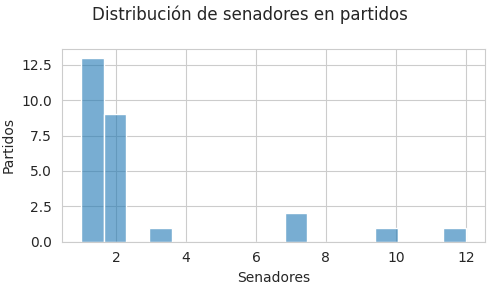
\includegraphics[scale=0.7]{../visualizations/distrib_histplot_senators_parties.png}
\caption{Distribución de senadores en partidos políticos.}
\label{fig-distrib-senators}
\end{figure}

Solo uno de los partidos (Frente de todos) cuenta con 12
senadores; también uno solo (Alianza frente para la victoria) es
representado por 10 senadores; dos partidos (Alianza cambiemos y
Juntos por el cambio) cuentan con 7 senadores, y el resto de los
partidos tienen entre 3, 2 y un senador.
En cuanto a las provincias (24 en total), todas tienen 3 senadores
exceptuando a Tucumán y a La Rioja, que tienen solo 2.

La figura \ref{fig-distrib-vote} nos muestra además que la intención
de voto no guarda una relación unívoca con los partidos a los cuales los
senadores representan. A excepción de los partidos que cuentan con un único
senador, la mayoría es representado con senadores que votaron a favor y senadores
que votaron en contra de la ley para el acceso al aborto. Aquí también
es posible ver que un senador del Frente Justicialista se abstuvo de votar,
mientras que dos senadores, uno de Cambiemos Fuerza Cívica Riojana y uno de
Frente Unidad Justicialista San Luis, estuvieron ausentes en la votación.

\begin{figure}[h!]
\centering
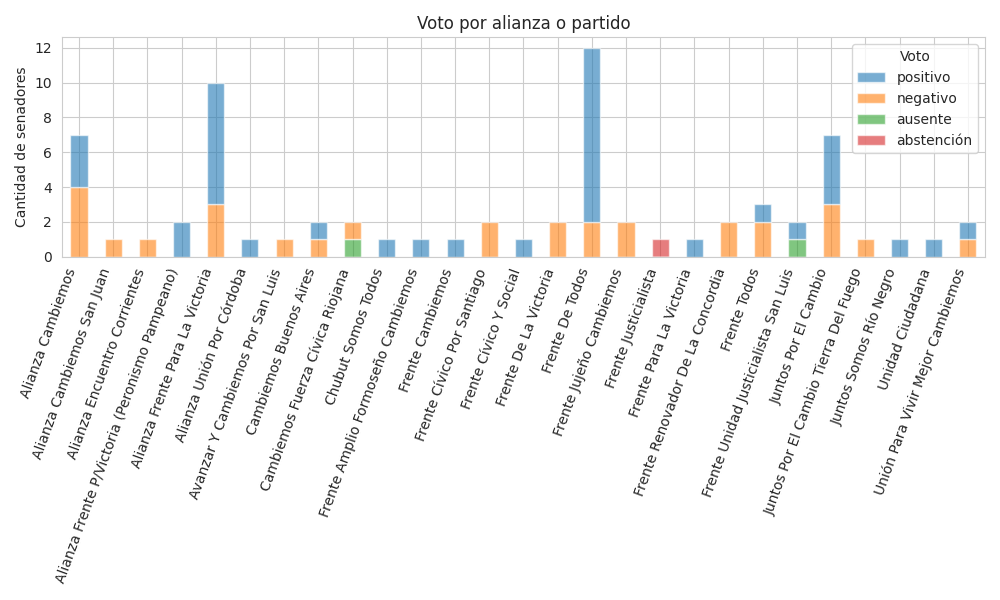
\includegraphics[scale=0.48]{../visualizations/senators_vote_by_party.png}
\caption{Distribución de votos en los distintos partidos políticos.}
\label{fig-distrib-vote}
\end{figure}

Respecto de las intervenciones discursivas, observamos que, en promedio, se emitieron
2.87 discursos por senador, con un desvío estándar de 6.23 y una mediana de 1, coincidente además
con la moda, lo que nos indicaría que se trata de una distribución asimétrica a derecha.
Estas medidas de centralidad incluyen a 9 senadores que no intervinieron en
la sesión, 7 de ellos votaron en contra de la despenalización del aborto; uno, a favor,
y uno estuvo ausente durante la votación. La figura \ref{fig-distrib-speech} muestra esta
distribución global y también discriminada por intención de voto.
Al desagregar los datos según elección en la votación, vemos que las abstenciones no presentan
dispersión y su media se ubica en el valor 1. Esto se debe a que solo un senador
se abstuvo de votar y, a su vez, solo emitió un discurso.
Una situación similar se da en las ausencias, donde también se observa un único discurso.
Pero dado que dos senadores estuvieron ausentes, la media se ubica hacia el valor 0.5 y
el desvío, hacia el 0.7.
En cuanto a los votos positivos y negativos, ambos presentan una moda de 1, pero los negativos
exhiben una media y un desvío estándar mayor que los positivos: $3.03\pm8.43$ \textit{versus} 
$2.92\pm4.26$, respectivamente. Ambos casos presentan obsrvaciones atípicas, pero en los votos
negativos estos casos muestran valores más extremos, por lo que la media y el desvío se
ven influenciados y adoptan también valores más altos.

\begin{figure}[h!]
    \centering
    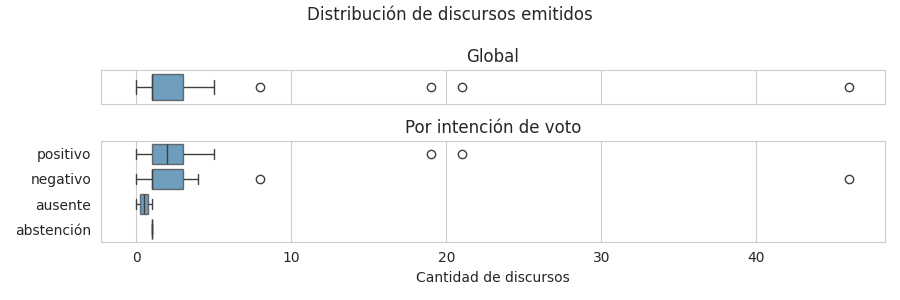
\includegraphics[scale=0.5]{../visualizations/speech_by_vote.png}
    \caption{Distribución de votos en los distintos partidos políticos.}
    \label{fig-distrib-speech}
\end{figure}

Por último, al hacer foco en la longitud de los discursos pronunciados, vemos que su
distribución varía dependiendo de si los medimos en \textit{tokens} totales o únicos.
Un \textit{token} es una secuencia de caracteres que queremos considerar como un
grupo\footnote{\citet*{bird2009natural}}. Aquí este grupo constituye lo que denominamos
`palabra'. En promedio, los discursos emitidos tienen 418 palabras, con un desvío
estándar de 714 palabras; la mediana es de 11 y la moda, de 7. Sin embargo, estas medidas
reflejan las palabras totales utilizadas en cada intervención, sin considerar si se repiten
o no: cada ocurrencia de una palabra cuenta, sin importar si ya fue pronunciada en el mismo
discurso. Es por eso que, a fines comparativos, se tomaron también las medidas de centralidad
de los \textit{tokens} únicos, las cuales mostraron una media de 161 palabras por discurso
con un desvío de 245, una mediana de 11 y una moda de 1. La figura \ref{fig-distrib-tokens}
refleja este contraste. Como es posible observar, si bien en ambos casos los discursos
muestran \textit{outliers} respecto de su longitud, cuando esta se mide en palabras
totales, presenta una mayor cantidad de casos atípicos con valores más extremos que
al medirla en \textit{tokens} únicos. En este último caso, un
$20\percentsign$ de los registros son \textit{outliers}, de los cuales solo el
$17\percentsign$ constituyen casos extremos, mientras que, al considerar
el total de palabras, un $22\percentsign$ de los datos resultan atípicos y,
de ellos, el $32\percentsign$ son extremos\footnote{Para este análisis se utilizó el
test de Tukey, que toma el rango intercuartil o \textit{IQR} (\textit{Q3-Q1}, donde
\textit{Q1} refiere al primer cuartil y \textit{Q3}, al terceo) y considera
valores atípicos leves a aquellos que se encuentran entre
$Q1 - (1.5 * IQR) < x < Q3 - (1.5 * IQR)$ y como extremos a los que están entre
$Q1 - (3 * IQR) < x < Q3 - (3 * IQR)$.}.
\todo[color=green!40,size=\tiny]{La longitud está menos delimitada, pero la temática
es específica. Entonces podría ser, cuando son tokens únicos no haya tanta dispersión
porque el tópico es uno y las palabras para referirnos a él están un poco más delimitadas
que la cantidad de veces que se puede usar una de estas mismas palabras al en un discurso.}

\begin{figure}[h!]
    \centering
    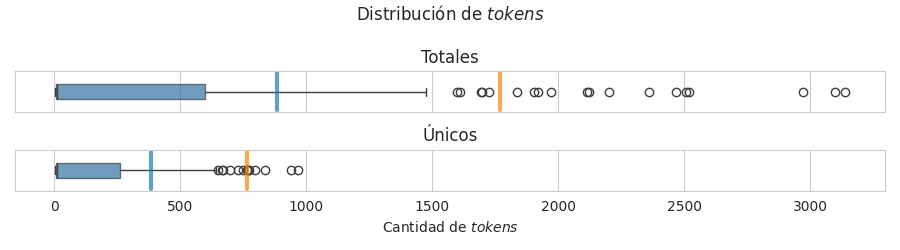
\includegraphics[scale=0.5]{../visualizations/distrib_tokens.png}
    \caption{Distribución de \textit{tokens} totales y únicos en los discursos pronunciados. En ambos gráficos,
    la línea azul indica el límite a partir del cual una observación se considera atípica leve
    ($IQR*1.5$) y la naranja, el límite a partir del cual se la considera atípica extrema ($IQR*3$).}
    \label{fig-distrib-tokens}
\end{figure}


%\begin{table}[ht]
%\centering
%\begin{tabular}{ |c|c|c|c|c| }
%    \hline
%    Voto & Media & Desvío & Mediana & Moda \\
%    \hline\hline
%    Abstención & 1.00 & 0.00 & 1.00 & 1 \\
%    \hline
%    Ausente & 0.50 & 0.71 & 0.50 & 0 \\
%    \hline
%    Negativo & 3.03 & 8.43 & 1.00 & 1 \\
%    \hline
%    Positivo & 2.92 & 4.26 & 2.00 & 1 \\
%    \hline
%\end{tabular}
%\caption{Medidas de centralidad de la cantidad de discursos emitidos}
%\label{table-tokens}
%\end{table}



\section{Metodolog\'ia}\label{section-methods}

\subsection{Anotación}\label{subsection-methods-annotation}
Para todas las categor\'ias de palabras se prefiere la lematizaci\'on. A continuaci\'on
se detallan las decisiones tomadas en casos particulares.

\subsubsection{Conectores}
Clases de palabra como preposiciones (`seg\'un'), pronombres relativos (`que') o
conjunciones (`si') que suelen funcionar como conectores subordinantes son
etiquetados con la categor\'ia \textit{SCONJ}.

\subsubsection{Nombres}
Por cuestiones de relevancia para el estudio, se mantiene la marca de g\'enero (femenino
o masculino), pero se omite la marca de n\'umero (singular o plural). Ejemplo: `abuelas'
$\rightarrow$ `abuela'.

\subsubsection{N\'umeros}
Se omiten todos, aquellos que aparecen en d\'igitos (`1', `10', etc.) y los que aparecen
en caracters (`cuarenta').

\subsubsection{Puntuaci\'on}
Se omiten todas los signos etiquetados como signos de puntuaci\'on (\textit{PUNCT}).
Ejemplos: `¿', `?', `;'.

\subsubsection{Verbos}
\begin{itemize}
    \item Se omiten los cl\'iticos (`la', `lo', `le' y sus formas plurales). En caso de
    que el verbo presente una forma con cl\'itico, se lo omite y se lo convierte a su
    forma infinitiva. Ejemplo: `consierar\textit{la}' $\rightarrow$ `consierar'.
    \item Se omiten las formas reflexivas (`se'). En caso de que el verbo presente
    una forma reflexiva, se lo omite y se lo convierte a su forma infinitiva.
    Ejemplo: `enfrentar\textit{se}' $\rightarrow$ `enfrentar'.
\end{itemize}

\subsubsection{Verbos auxiliares}
\begin{itemize}
    \item La categor\'ia \textit{AUX} es despreciada.
    \item Aquellos verbos catalogados con la etiqueta \textit{AUX} fueron
    recatalogados como verbos (\textit{VERB}) si pertenecen a ese tipo de
    palabra, y transformados a la forma en infinitivo. Ejemplo: `seamos' $\rightarrow$ `ser'.
\end{itemize}

\subsubsection{Palabras con tokenizados err\'oneos}
Se omiten las cadenas de caracteres que al ser tokenizadas quedaron unidas a un
signo de puntuaci\'on. Ejemplos: `¡negando', `¿por'.


\subsection{Selección de rasgos}\label{subsection-methods-features}
Tomando como referencia las t\'ecnicas estad\'isticas descriptas por
\cite{monroe2008fightin}, se implementaron vectorizadores que, a partir de
recibir una lista de documentos, devolviesen una matriz donde cada fila
representase un documento y cada columna, una palabra. Los valores
reflejados en las celdas de esa matriz corresponden a la frecuencia absoluta
de la palabra en el docuemnto en cuesti\'on. Lo que diferencia a
las distintas matrices es el conjunto de palabras seleccionadas
para ser usadas como componentes del vector
que caracteriza a los documentos. Cada vectorizador utiliza
una t\'ecnica estad\'istica determinada para obtener las \textit{N}
palabras m\'as representativas del grupo de votantes a favor y
en contra de la legalizaci\'on del aborto, donde \textit{N} es el n\'umero
entero positivo que indica la cantidad de palabras a considerar.
Los detalles particulares de cada
t\'ecnica pueden encontrarse en la secci\'on \ref{subsubsec-methods-vectorizers}.
\par
Para la implementaci\'on se tom\'o como base el estimador \texttt{CountVectorizer}
de la librer\'ia \textit{scikit-learn}, de modo que las clases u objetos resultantes
contasen con los mismos m\'etodos y, luego, pudieran ser utilizadas en un
\textit{pipeline}
de trabajo definido con clases y m\'etodos de la misma librer\'ia.
\par
En primer lugar, se separ\'o el \textit{dataset} en un conjunto de entrenamiento
y otro de testeo ($80\percentsign$ y $20\percentsign$ de los datos, respectivamente).
En esta divisi\'on se tuvo en cuenta la variable \textit{target} \texttt{voto} de modo
que los subconjuntos obtenidos reflejasen la misma proporci\'on de votos a favor
y en contra. Asimismo, se us\'o una semilla para garantizar que los resultados
fuesen replicables. La variable objetivo, adem\'as, fue codificada a valores
num\'ericos para poder ser utilizada por los algoritmos de predicci\'on.
\par
Luego, tomando solamente el conjunto de entrenamiento y vectorizando
previamente los datos con cada uno de los vectorizadores desarrollados,
se entren\'o una Regresi\'on Log\'istica utilizando los par\'ametros por defecto
de la librer\'ia \textit{scikit-learn}
\footnote{Entre los m\'as relevantes para este trabajo, destacamos: regularizaci\'on
o \texttt{penalty=l2}, intensidad inversa de la regularizaci\'on o \texttt{C=1},
ajuste de \textit{bias} o \texttt{fit\_intercept=True} y peso de cada clases
o \texttt{class\_weight=None}.
Para m\'as informaci\'on sobre los par\'ametros por defecto, consultar:
\url{https://scikit-learn.org/1.5/modules/generated/sklearn.linear_model.LogisticRegression.html} [\'ultimo acceso: 15--10--2024]}.
En cada entrenamiento se aplic\'o el m\'etodo
de validac\'on cruzada con 5 subconjuntos: 4 para entrenamiento y 1 para testeo
en cada iteraci\'on.
Para esto, al igual que en la primera divisi\'on, se cuid\'o de realizar
una segmentaci\'on estratificada, utilizar una semilla y
aplicar la misma segmentaci\'on en cada vectorizador,
de modo que las circunstancias de evaluaci\'on fuesen lo m\'as semejantes posible
y eso permitiese comparar qu\'e vectorizadores conducen a un mejor entrenamiento.
La tabla \ref{table-methods-vectorizers} resume las combinaciones testeadas
en la experimentaci\'on. En todos los casos se generaron vectores de trescientas
($300$) dimensiones.

\begin{table}[ht]
\centering
\begin{tabular}{ |c|c|c|c|c| }
    \hline
    T\'ecnica & \textit{Remoci\'on de stopwords} & \textit{Log} & Suavizado \\
    \hline\hline
    Frecuencias absolutas & No & No & No \\
    \hline
    Proporciones & No & No & No \\
    \hline
    Proporciones & S\'i (NLTK) & No & No \\
    \hline
    Proporciones & S\'i (Zipf) & No & No \\
    \hline
    \textit{Ratio} de \textit{odds} & No & No & No \\
    \hline
    \textit{Ratio} de \textit{odds} & No & S\'i (\textit{odds}) & No \\
    \hline
    \textit{Ratio} de \textit{odds} & No & S\'i (\textit{odds}) & S\'i ($0.5$) \\
    \hline
    \textit{TF-IDF} & No & No & No \\
    \hline
    \textit{TF-IDF} & No & S\'i (\textit{IDF}) & No \\
    \hline
    \textit{Word scores} & No & No & No \\
    \hline
\end{tabular}
\caption{T\'ecnicas estad\'isticas testeadas para la vectorizaci\'on de los
discursos utilizados en el entrenamiento del modelo de Regresi\'on Log\'isitca.}
\label{table-methods-vectorizers}
\end{table}

\subsubsection{M\'etodos estad\'isticos utilizados en la vectorizaci\'on de documentos}
\label{subsubsec-methods-vectorizers}

De los m\'etodos aplicados, dos (\textit{TF-IDF} y \textit{Word Scores}) consisten
en algoritmos para la asignaci\'on de puntuaciones o \textit{scores} a los
palabras dentro de un \textit{corpus}. El resto de las t\'ecnicas emplean
m\'etricas estad\'isticas sencillas. Para la aplicaci\'on de estos procedimientos
se utiliz\'o como \textit{token} las lematizaciones de las palabras incluyendo
su categor\'ia gramatical\footnote{Para esto, todos los documentos fueron
pre{--}procesados de modo tal que cada palabra fue reemplazada por un
\textit{token} construido de la siguiente forma:
$\langle lema \rangle\_ \langle \textit{POS tag} \rangle$, donde
$\langle lema \rangle$ refiere al lema de la palabra y
$\langle \textit{POS tag} \rangle$, a su etiqueta \textit{POS}.}.


\paragraph{Diferencia de frecuencias absolutas}
\label{paragraph-methods-freq-abs}
Este m\'etodo utiliza la diferencia de frecuencias absolutas de los \textit{tokens} entre
los discursos de ambos grupos para extraer el conjunto m\'as representativo de
cada uno:

\begin{equation}
y_t = y_{t}^{(P)}-y_{t}^{(N)}
\end{equation}

donde $y_{t}^{(X)}$ refiere a la cantidad de ocurrencias absolutas del \textit{token}
\textit{t} en los discursos que votaron de manera positiva
(si $X=P$) y negativa (cuando $X=N$).
En los casos en los que $y_{t}$ sea mayor o igual a $0$, el \textit{token} $t$
ser\'a caracter\'istico del discurso de los senadores que votaron a favor de
la legalizaci\'on. En caso contrario, ser\'a caracter\'istico de quienes votaron
en contra.
De este modo, se seleccionaron las trescientas dimensiones m\'as representativas de
ambos grupos cuidando que hubiese igual cantidad de \textit{tokens} para cada uno.
Un procedimiento an\'alogo es aplicado en el resto de las t\'ecnicas pero utilizando
un criterio de contrastaci\'on distinto en cada caso.

\paragraph{Diferencia de proporciones}
\label{paragraph-methods-proportions}
El segundo contraste utiliza la proporci\'on de \textit{tokens}
en cada conjunto de discursos.

\begin{equation}
    f_t = f_{t}^{(P)}-f_{t}^{(N)}
\end{equation}


donde $f_{t}^{(X)}$ se define como $y_{t}^{(X)} / n^{(X)}$, siendo $y_{t}^{(X)}$
la frecuencia absoluta del \textit{token} $t$ en el cojunto los discursos de $X$
y $n^{(X)}$, la cantidad de \textit{tokens} totales en esos discursos.

\subparagraph{Remoci\'on de \textit{stopwords}}
\label{paragraph-methods-proportions-stopwords}
Tambi\'en se intent\'o calcular la diferencia de proporciones removiendo
previamente los \textit{tokens} considerados \textit{stopwords}.
Para esto se probaron dos alternativas.
Por un lado, se utiliz\'o el conjunto predefinido de la librer\'ia \textit{NLTK}
\footnote{\url{https://raw.githubusercontent.com/nltk/nltk_data/gh-pages/packages/corpora/stopwords.zip} [\'ultimo acceso: 15--10--2024]}
y, por otro, la Ley de Zipf.
Este \'ultimo procedimiento consiste en calcular la frecuencia absoluta de aparici\'on de
cada \textit{token} y, en virtud de ella, establecer un \textit{ranking}
orden\'andolos de manera decreciente.
Luego, se contrasta dicha frecuencia con el orden asignado y se define
un umbral a partir del cual una palabra es considerada \textit{stopword}.
Resulta pertinente notar que, dado que la frecuencia absoluta de aparici\'on
de una palabra se determina en relaci\'on al conjunto de documentos en el cual
esta frecuencia es medida, las diferentes iteraciones de la validaci\'on cruzada
generaron distintos conjuntos de \textit{stopwrods}.
En todas las iteraciones se removieron $100$ \textit{tokens} seleccionados
con este m\'etodo. Este n\'umero fue seleccionado tras realizar un an\'alisis del
conjunto de datos completo como primera aproximaci\'on general (ver secci\'on
\ref{appendix-plots-zipf-law}.).

\paragraph{\textit{Ratio} de \textit{Odds}}
Se utilizan \textit{odds} de ambos conjuntos de discursos como
t\'ecnica de selecci\'on. En este caso, los \textit{tokens} m\'as caracter\'isticos
no resultan de una diferencia sino de un cociente:

\begin{equation}
    O_{t} = \frac{O_{t}^{(P)}}{O_{t}^{(N)}}
\end{equation}

aqu\'i, $O_{t}^{(X)}$ consiste en $f_{t}^{(X)}/(1-f_{t}^{(X)})$.
Otra diferencia entre esta t\'ecnica y el resto es que aqu\'i el punto de
corte para considerar a un \textit{token} como caracter\'istico de
determinado grupo de discursos no es el $0$ sino el $1$, por la misma
definici\'on de la funci\'on.

\paragraph{\textit{Ratio} \textit{Log-odds}}
Sobre los \textit{odds}, tambi\'en se calcul\'o el \textit{ratio log-odds}.
Para este c\'alculo se utiliz\'o el logaritmo natural: $\ln{O_t}$.
Asimismo, se realiz\'o un suavizado sobre las frecuencias en los casos
en los que los \textit{tokens} solo se encontraban en uno de los grupos
discursivos. Dicho suavizado consisti\'o en agregar un peso predefinido a las
frecuencias relativas, $\tilde{f}^{i}_{w} = f^{i}_{w}+\epsilon$, y tomar
este valor en el c\'alculo del \textit{ratio}. Siguiendo a \cite{monroe2008fightin},
se utiliz\'o $\epsilon=0.5$.

\paragraph{\textit{TF-IDF}}
\label{paragraph-methods-tfidf}
Si bien la librer\'ia \textit{scikit-learn} cuenta con un vectorizador
que permite calcular los \textit{scores} de \textit{TF-IDF}
\footnote{Para m\'as informaci\'on sobre las f\'ormulas
implementadas por \textit{scikit-learn}, visitar:
\url{https://scikit-learn.org/stable/modules/feature_extraction.html\#tfidf-term-weighting} [\'ultimo acceso: 15--10--2024].},
dado que la f\'ormula propuesta por \Citeauthor{monroe2008fightin} plantea
algunas modificaciones a dicha implementaci\'on, se decidi\'o
desarrollar un vectorizador propio para obtener un resultado
m\'as aproximado al descripto por los autores, quienes indican haber usado
dos f\'ormulas diferentes: ambas emplean la frecuencia
de t\'ermino natural y sin normalizar, pero una con la frecuencia de documentos
con logaritmo (f\'ormula \ref{equation-tfidf-ntn}) y la otra, con la frecuencia
de documentos natural (f\'ormula \ref{equation-tfidf-nnn}).

\begin{equation}
\label{equation-tfidf-ntn}
    tf.idf_{t}^{(X)}(ntn) = f_{t}^{(X)} \times \ln\bigg({\frac{1}{df_{t}}}\bigg)
\end{equation}

\begin{equation}
\label{equation-tfidf-nnn}
    tf.idf_{t}^{(X)}(nnn) = \frac{f_{t}^{(X)}}{df_{t}}
\end{equation}

donde $f_{t}^{X}$ refiere a la proporci\'on del \textit{token} $t$
en el discurso perteneciente a $X$
(con $X \in \lbrace P,N \rbrace$) y $df_t$, a la cantidad
de documentos totales en los que ese \textit{token} aparece.
\par
Lo que los autores no mencionan es qu\'e tipo de comparaci\'on realizan
entre los \textit{tokens} pertenecientes a los distintos discursos.
Siguiendo los procedimientos anteriores, en este trabajo se opt\'o por usar
la sustracci\'on, por lo que:

\begin{equation*}
    tf.idf_{t} = tf.idf_{t}^{P}-tf.idf_{t}^{N}
\end{equation*}

\paragraph{\textit{Word Scores}}
\label{paragraph-methods-wordscores}
Por \'ultimo, este procedimiento le asigna un peso a los \textit{tokens}
a partir del siguiente c\'alculo:

\begin{equation*}
    W_{t}^{^*(P-N)} = \frac{
        y_{t}^{(P)}/n^{(P)}-y_{t}^{(N)}/n^{(N)}
        }{
            y_{t}^{(P)}/n^{(P)}+y_{t}^{(N)}/n^{(N)}
        }n_{t}
\end{equation*}

donde $y_{t}^{(X)}$ refiere a la frecuencia absoluta
del grupo $X$ y $n^{(X)}$, a la cantidad de \textit{tokens} totales en $X$.


\subsection{Entrenamiento de un modelo predictivo}\label{subsection-methods-models}
%% Clasificaci\'on ==> w1: 0.004, w2: 0.002
%   - RF

\subsection{Evaluaci\'on}\label{subsection-methods-evaluation}
\input{sections/methods/evaluation.tex}


\section{Resultados}\label{section-results}

\subsection{Anotación}\label{subsec-results-annotation}
Para todas las categor\'ias de palabras se prefiere la lematizaci\'on. A continuaci\'on
se detallan las decisiones tomadas en casos particulares.

\subsubsection{Conectores}
Clases de palabra como preposiciones (`seg\'un'), pronombres relativos (`que') o
conjunciones (`si') que suelen funcionar como conectores subordinantes son
etiquetados con la categor\'ia \textit{SCONJ}.

\subsubsection{Nombres}
Por cuestiones de relevancia para el estudio, se mantiene la marca de g\'enero (femenino
o masculino), pero se omite la marca de n\'umero (singular o plural). Ejemplo: `abuelas'
$\rightarrow$ `abuela'.

\subsubsection{N\'umeros}
Se omiten todos, aquellos que aparecen en d\'igitos (`1', `10', etc.) y los que aparecen
en caracters (`cuarenta').

\subsubsection{Puntuaci\'on}
Se omiten todas los signos etiquetados como signos de puntuaci\'on (\textit{PUNCT}).
Ejemplos: `¿', `?', `;'.

\subsubsection{Verbos}
\begin{itemize}
    \item Se omiten los cl\'iticos (`la', `lo', `le' y sus formas plurales). En caso de
    que el verbo presente una forma con cl\'itico, se lo omite y se lo convierte a su
    forma infinitiva. Ejemplo: `consierar\textit{la}' $\rightarrow$ `consierar'.
    \item Se omiten las formas reflexivas (`se'). En caso de que el verbo presente
    una forma reflexiva, se lo omite y se lo convierte a su forma infinitiva.
    Ejemplo: `enfrentar\textit{se}' $\rightarrow$ `enfrentar'.
\end{itemize}

\subsubsection{Verbos auxiliares}
\begin{itemize}
    \item La categor\'ia \textit{AUX} es despreciada.
    \item Aquellos verbos catalogados con la etiqueta \textit{AUX} fueron
    recatalogados como verbos (\textit{VERB}) si pertenecen a ese tipo de
    palabra, y transformados a la forma en infinitivo. Ejemplo: `seamos' $\rightarrow$ `ser'.
\end{itemize}

\subsubsection{Palabras con tokenizados err\'oneos}
Se omiten las cadenas de caracteres que al ser tokenizadas quedaron unidas a un
signo de puntuaci\'on. Ejemplos: `¡negando', `¿por'.


\subsection{Selección de rasgos}\label{subsection-results-features}
Tomando como referencia las t\'ecnicas estad\'isticas descriptas por
\cite{monroe2008fightin}, se implementaron vectorizadores que, a partir de
recibir una lista de documentos, devolviesen una matriz donde cada fila
representase un documento y cada columna, una palabra. Los valores
reflejados en las celdas de esa matriz corresponden a la frecuencia absoluta
de la palabra en el docuemnto en cuesti\'on. Lo que diferencia a
las distintas matrices es el conjunto de palabras seleccionadas
para ser usadas como componentes del vector
que caracteriza a los documentos. Cada vectorizador utiliza
una t\'ecnica estad\'istica determinada para obtener las \textit{N}
palabras m\'as representativas del grupo de votantes a favor y
en contra de la legalizaci\'on del aborto, donde \textit{N} es el n\'umero
entero positivo que indica la cantidad de palabras a considerar.
Los detalles particulares de cada
t\'ecnica pueden encontrarse en la secci\'on \ref{subsubsec-methods-vectorizers}.
\par
Para la implementaci\'on se tom\'o como base el estimador \texttt{CountVectorizer}
de la librer\'ia \textit{scikit-learn}, de modo que las clases u objetos resultantes
contasen con los mismos m\'etodos y, luego, pudieran ser utilizadas en un
\textit{pipeline}
de trabajo definido con clases y m\'etodos de la misma librer\'ia.
\par
En primer lugar, se separ\'o el \textit{dataset} en un conjunto de entrenamiento
y otro de testeo ($80\percentsign$ y $20\percentsign$ de los datos, respectivamente).
En esta divisi\'on se tuvo en cuenta la variable \textit{target} \texttt{voto} de modo
que los subconjuntos obtenidos reflejasen la misma proporci\'on de votos a favor
y en contra. Asimismo, se us\'o una semilla para garantizar que los resultados
fuesen replicables. La variable objetivo, adem\'as, fue codificada a valores
num\'ericos para poder ser utilizada por los algoritmos de predicci\'on.
\par
Luego, tomando solamente el conjunto de entrenamiento y vectorizando
previamente los datos con cada uno de los vectorizadores desarrollados,
se entren\'o una Regresi\'on Log\'istica utilizando los par\'ametros por defecto
de la librer\'ia \textit{scikit-learn}
\footnote{Entre los m\'as relevantes para este trabajo, destacamos: regularizaci\'on
o \texttt{penalty=l2}, intensidad inversa de la regularizaci\'on o \texttt{C=1},
ajuste de \textit{bias} o \texttt{fit\_intercept=True} y peso de cada clases
o \texttt{class\_weight=None}.
Para m\'as informaci\'on sobre los par\'ametros por defecto, consultar:
\url{https://scikit-learn.org/1.5/modules/generated/sklearn.linear_model.LogisticRegression.html} [\'ultimo acceso: 15--10--2024]}.
En cada entrenamiento se aplic\'o el m\'etodo
de validac\'on cruzada con 5 subconjuntos: 4 para entrenamiento y 1 para testeo
en cada iteraci\'on.
Para esto, al igual que en la primera divisi\'on, se cuid\'o de realizar
una segmentaci\'on estratificada, utilizar una semilla y
aplicar la misma segmentaci\'on en cada vectorizador,
de modo que las circunstancias de evaluaci\'on fuesen lo m\'as semejantes posible
y eso permitiese comparar qu\'e vectorizadores conducen a un mejor entrenamiento.
La tabla \ref{table-methods-vectorizers} resume las combinaciones testeadas
en la experimentaci\'on. En todos los casos se generaron vectores de trescientas
($300$) dimensiones.

\begin{table}[ht]
\centering
\begin{tabular}{ |c|c|c|c|c| }
    \hline
    T\'ecnica & \textit{Remoci\'on de stopwords} & \textit{Log} & Suavizado \\
    \hline\hline
    Frecuencias absolutas & No & No & No \\
    \hline
    Proporciones & No & No & No \\
    \hline
    Proporciones & S\'i (NLTK) & No & No \\
    \hline
    Proporciones & S\'i (Zipf) & No & No \\
    \hline
    \textit{Ratio} de \textit{odds} & No & No & No \\
    \hline
    \textit{Ratio} de \textit{odds} & No & S\'i (\textit{odds}) & No \\
    \hline
    \textit{Ratio} de \textit{odds} & No & S\'i (\textit{odds}) & S\'i ($0.5$) \\
    \hline
    \textit{TF-IDF} & No & No & No \\
    \hline
    \textit{TF-IDF} & No & S\'i (\textit{IDF}) & No \\
    \hline
    \textit{Word scores} & No & No & No \\
    \hline
\end{tabular}
\caption{T\'ecnicas estad\'isticas testeadas para la vectorizaci\'on de los
discursos utilizados en el entrenamiento del modelo de Regresi\'on Log\'isitca.}
\label{table-methods-vectorizers}
\end{table}

\subsubsection{M\'etodos estad\'isticos utilizados en la vectorizaci\'on de documentos}
\label{subsubsec-methods-vectorizers}

De los m\'etodos aplicados, dos (\textit{TF-IDF} y \textit{Word Scores}) consisten
en algoritmos para la asignaci\'on de puntuaciones o \textit{scores} a los
palabras dentro de un \textit{corpus}. El resto de las t\'ecnicas emplean
m\'etricas estad\'isticas sencillas. Para la aplicaci\'on de estos procedimientos
se utiliz\'o como \textit{token} las lematizaciones de las palabras incluyendo
su categor\'ia gramatical\footnote{Para esto, todos los documentos fueron
pre{--}procesados de modo tal que cada palabra fue reemplazada por un
\textit{token} construido de la siguiente forma:
$\langle lema \rangle\_ \langle \textit{POS tag} \rangle$, donde
$\langle lema \rangle$ refiere al lema de la palabra y
$\langle \textit{POS tag} \rangle$, a su etiqueta \textit{POS}.}.


\paragraph{Diferencia de frecuencias absolutas}
\label{paragraph-methods-freq-abs}
Este m\'etodo utiliza la diferencia de frecuencias absolutas de los \textit{tokens} entre
los discursos de ambos grupos para extraer el conjunto m\'as representativo de
cada uno:

\begin{equation}
y_t = y_{t}^{(P)}-y_{t}^{(N)}
\end{equation}

donde $y_{t}^{(X)}$ refiere a la cantidad de ocurrencias absolutas del \textit{token}
\textit{t} en los discursos que votaron de manera positiva
(si $X=P$) y negativa (cuando $X=N$).
En los casos en los que $y_{t}$ sea mayor o igual a $0$, el \textit{token} $t$
ser\'a caracter\'istico del discurso de los senadores que votaron a favor de
la legalizaci\'on. En caso contrario, ser\'a caracter\'istico de quienes votaron
en contra.
De este modo, se seleccionaron las trescientas dimensiones m\'as representativas de
ambos grupos cuidando que hubiese igual cantidad de \textit{tokens} para cada uno.
Un procedimiento an\'alogo es aplicado en el resto de las t\'ecnicas pero utilizando
un criterio de contrastaci\'on distinto en cada caso.

\paragraph{Diferencia de proporciones}
\label{paragraph-methods-proportions}
El segundo contraste utiliza la proporci\'on de \textit{tokens}
en cada conjunto de discursos.

\begin{equation}
    f_t = f_{t}^{(P)}-f_{t}^{(N)}
\end{equation}


donde $f_{t}^{(X)}$ se define como $y_{t}^{(X)} / n^{(X)}$, siendo $y_{t}^{(X)}$
la frecuencia absoluta del \textit{token} $t$ en el cojunto los discursos de $X$
y $n^{(X)}$, la cantidad de \textit{tokens} totales en esos discursos.

\subparagraph{Remoci\'on de \textit{stopwords}}
\label{paragraph-methods-proportions-stopwords}
Tambi\'en se intent\'o calcular la diferencia de proporciones removiendo
previamente los \textit{tokens} considerados \textit{stopwords}.
Para esto se probaron dos alternativas.
Por un lado, se utiliz\'o el conjunto predefinido de la librer\'ia \textit{NLTK}
\footnote{\url{https://raw.githubusercontent.com/nltk/nltk_data/gh-pages/packages/corpora/stopwords.zip} [\'ultimo acceso: 15--10--2024]}
y, por otro, la Ley de Zipf.
Este \'ultimo procedimiento consiste en calcular la frecuencia absoluta de aparici\'on de
cada \textit{token} y, en virtud de ella, establecer un \textit{ranking}
orden\'andolos de manera decreciente.
Luego, se contrasta dicha frecuencia con el orden asignado y se define
un umbral a partir del cual una palabra es considerada \textit{stopword}.
Resulta pertinente notar que, dado que la frecuencia absoluta de aparici\'on
de una palabra se determina en relaci\'on al conjunto de documentos en el cual
esta frecuencia es medida, las diferentes iteraciones de la validaci\'on cruzada
generaron distintos conjuntos de \textit{stopwrods}.
En todas las iteraciones se removieron $100$ \textit{tokens} seleccionados
con este m\'etodo. Este n\'umero fue seleccionado tras realizar un an\'alisis del
conjunto de datos completo como primera aproximaci\'on general (ver secci\'on
\ref{appendix-plots-zipf-law}.).

\paragraph{\textit{Ratio} de \textit{Odds}}
Se utilizan \textit{odds} de ambos conjuntos de discursos como
t\'ecnica de selecci\'on. En este caso, los \textit{tokens} m\'as caracter\'isticos
no resultan de una diferencia sino de un cociente:

\begin{equation}
    O_{t} = \frac{O_{t}^{(P)}}{O_{t}^{(N)}}
\end{equation}

aqu\'i, $O_{t}^{(X)}$ consiste en $f_{t}^{(X)}/(1-f_{t}^{(X)})$.
Otra diferencia entre esta t\'ecnica y el resto es que aqu\'i el punto de
corte para considerar a un \textit{token} como caracter\'istico de
determinado grupo de discursos no es el $0$ sino el $1$, por la misma
definici\'on de la funci\'on.

\paragraph{\textit{Ratio} \textit{Log-odds}}
Sobre los \textit{odds}, tambi\'en se calcul\'o el \textit{ratio log-odds}.
Para este c\'alculo se utiliz\'o el logaritmo natural: $\ln{O_t}$.
Asimismo, se realiz\'o un suavizado sobre las frecuencias en los casos
en los que los \textit{tokens} solo se encontraban en uno de los grupos
discursivos. Dicho suavizado consisti\'o en agregar un peso predefinido a las
frecuencias relativas, $\tilde{f}^{i}_{w} = f^{i}_{w}+\epsilon$, y tomar
este valor en el c\'alculo del \textit{ratio}. Siguiendo a \cite{monroe2008fightin},
se utiliz\'o $\epsilon=0.5$.

\paragraph{\textit{TF-IDF}}
\label{paragraph-methods-tfidf}
Si bien la librer\'ia \textit{scikit-learn} cuenta con un vectorizador
que permite calcular los \textit{scores} de \textit{TF-IDF}
\footnote{Para m\'as informaci\'on sobre las f\'ormulas
implementadas por \textit{scikit-learn}, visitar:
\url{https://scikit-learn.org/stable/modules/feature_extraction.html\#tfidf-term-weighting} [\'ultimo acceso: 15--10--2024].},
dado que la f\'ormula propuesta por \Citeauthor{monroe2008fightin} plantea
algunas modificaciones a dicha implementaci\'on, se decidi\'o
desarrollar un vectorizador propio para obtener un resultado
m\'as aproximado al descripto por los autores, quienes indican haber usado
dos f\'ormulas diferentes: ambas emplean la frecuencia
de t\'ermino natural y sin normalizar, pero una con la frecuencia de documentos
con logaritmo (f\'ormula \ref{equation-tfidf-ntn}) y la otra, con la frecuencia
de documentos natural (f\'ormula \ref{equation-tfidf-nnn}).

\begin{equation}
\label{equation-tfidf-ntn}
    tf.idf_{t}^{(X)}(ntn) = f_{t}^{(X)} \times \ln\bigg({\frac{1}{df_{t}}}\bigg)
\end{equation}

\begin{equation}
\label{equation-tfidf-nnn}
    tf.idf_{t}^{(X)}(nnn) = \frac{f_{t}^{(X)}}{df_{t}}
\end{equation}

donde $f_{t}^{X}$ refiere a la proporci\'on del \textit{token} $t$
en el discurso perteneciente a $X$
(con $X \in \lbrace P,N \rbrace$) y $df_t$, a la cantidad
de documentos totales en los que ese \textit{token} aparece.
\par
Lo que los autores no mencionan es qu\'e tipo de comparaci\'on realizan
entre los \textit{tokens} pertenecientes a los distintos discursos.
Siguiendo los procedimientos anteriores, en este trabajo se opt\'o por usar
la sustracci\'on, por lo que:

\begin{equation*}
    tf.idf_{t} = tf.idf_{t}^{P}-tf.idf_{t}^{N}
\end{equation*}

\paragraph{\textit{Word Scores}}
\label{paragraph-methods-wordscores}
Por \'ultimo, este procedimiento le asigna un peso a los \textit{tokens}
a partir del siguiente c\'alculo:

\begin{equation*}
    W_{t}^{^*(P-N)} = \frac{
        y_{t}^{(P)}/n^{(P)}-y_{t}^{(N)}/n^{(N)}
        }{
            y_{t}^{(P)}/n^{(P)}+y_{t}^{(N)}/n^{(N)}
        }n_{t}
\end{equation*}

donde $y_{t}^{(X)}$ refiere a la frecuencia absoluta
del grupo $X$ y $n^{(X)}$, a la cantidad de \textit{tokens} totales en $X$.


\subsection{Entrenamiento de un modelo predictivo}\label{subsection-results-models}
%%% Clasificaci\'on ==> w1: 0.004, w2: 0.002
%   - RF

\subsection{Evaluaci\'on}\label{subsection-results-evaluation}
\input{sections/results/evaluation.tex}


\section{Discusi\'on y conclusiones}\label{section-discussion}

\bibliographystyle{linquiry3}
\bibliography{bibliography}

\clearpage
\appendix
\section{Anexo}\label{appendix}

\subsection{Guía de anotación}\label{appendix-annotation}
Para todas las categor\'ias de palabras se prefiere la lematizaci\'on. A continuaci\'on
se detallan las decisiones tomadas en casos particulares.

\subsubsection{Conectores}
Clases de palabra como preposiciones (`seg\'un'), pronombres relativos (`que') o
conjunciones (`si') que suelen funcionar como conectores subordinantes son
etiquetados con la categor\'ia \textit{SCONJ}.

\subsubsection{Nombres}
Por cuestiones de relevancia para el estudio, se mantiene la marca de g\'enero (femenino
o masculino), pero se omite la marca de n\'umero (singular o plural). Ejemplo: `abuelas'
$\rightarrow$ `abuela'.

\subsubsection{N\'umeros}
Se omiten todos, aquellos que aparecen en d\'igitos (`1', `10', etc.) y los que aparecen
en caracters (`cuarenta').

\subsubsection{Puntuaci\'on}
Se omiten todas los signos etiquetados como signos de puntuaci\'on (\textit{PUNCT}).
Ejemplos: `¿', `?', `;'.

\subsubsection{Verbos}
\begin{itemize}
    \item Se omiten los cl\'iticos (`la', `lo', `le' y sus formas plurales). En caso de
    que el verbo presente una forma con cl\'itico, se lo omite y se lo convierte a su
    forma infinitiva. Ejemplo: `consierar\textit{la}' $\rightarrow$ `consierar'.
    \item Se omiten las formas reflexivas (`se'). En caso de que el verbo presente
    una forma reflexiva, se lo omite y se lo convierte a su forma infinitiva.
    Ejemplo: `enfrentar\textit{se}' $\rightarrow$ `enfrentar'.
\end{itemize}

\subsubsection{Verbos auxiliares}
\begin{itemize}
    \item La categor\'ia \textit{AUX} es despreciada.
    \item Aquellos verbos catalogados con la etiqueta \textit{AUX} fueron
    recatalogados como verbos (\textit{VERB}) si pertenecen a ese tipo de
    palabra, y transformados a la forma en infinitivo. Ejemplo: `seamos' $\rightarrow$ `ser'.
\end{itemize}

\subsubsection{Palabras con tokenizados err\'oneos}
Se omiten las cadenas de caracteres que al ser tokenizadas quedaron unidas a un
signo de puntuaci\'on. Ejemplos: `¡negando', `¿por'.


\subsection{Gráficos adicionales}\label{appendix-plots}
Aqu\'i pueden encontrarse gr\'aficos adicionales sobre los m\'etodos empleados
en este trabajo.

\subsubsection{Ley de Zipf}
\label{appendix-plots-zipf-law}

\begin{figure}[!htb]
    \centering
    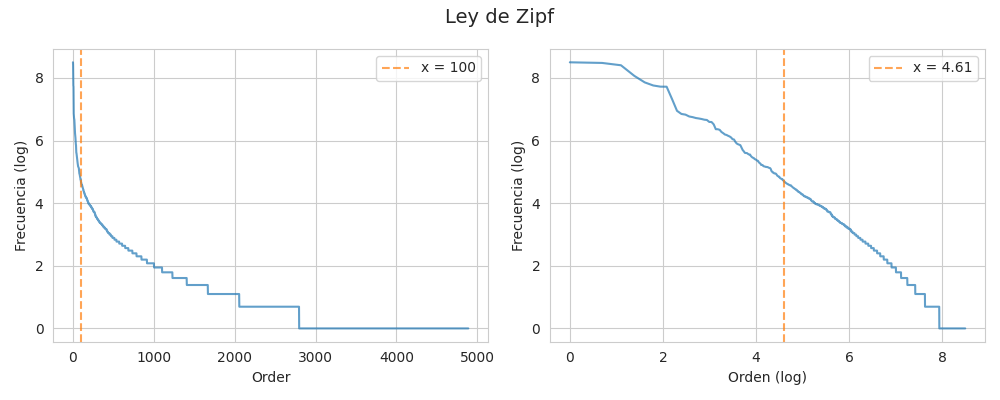
\includegraphics[scale=0.4]{../visualizations/ley_de_zipf.png}
    \caption{Contraste entre la frecuencia absoluta de cada palabra (en logaritmo)
    y el \textit{ranking} de esa palabra seg\'un su frecuencia. El gr\'afico de la
    izquierda exhibe el orden natural de cada palabra y el de la derecha, su logaritmo.
    En ambos casos, la l\'inea punteada naranja indica el umbral
    para considerar \textit{stopword} a una palabra.}
    \label{fig-zipf-law}
\end{figure}
\FloatBarrier

\subsubsection{Selecci\'on de vectorizador}
\label{appendix-plots-vectorizers}

\begin{figure}[!htb]
    \centering
    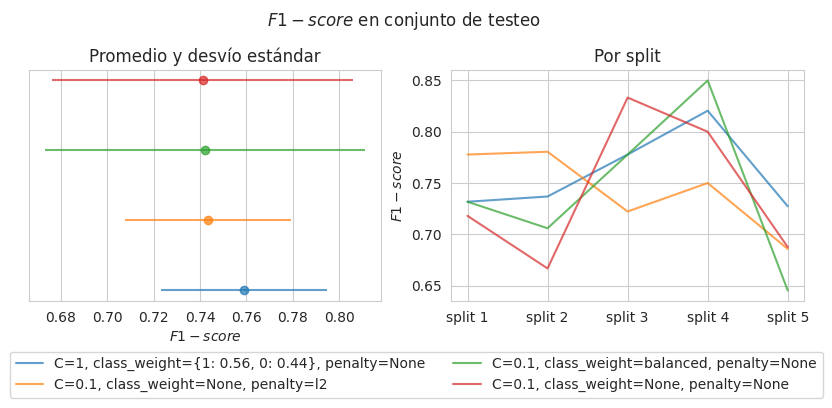
\includegraphics[scale=0.4]{../visualizations/features/f1_by_split.png}
    \caption{\textit{F1} por split de validaci\'on cruzada para el conjunto
    de entrenmiento y de testeo, para todos los vectorizadores en evaluaci\'on.}
    \label{fig-vectorizers-f1}
\end{figure}
\FloatBarrier

\begin{figure}[!htb]
    \centering
    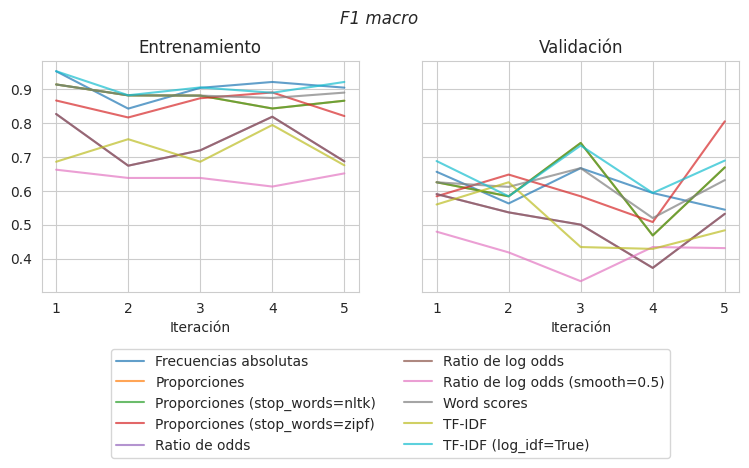
\includegraphics[scale=0.4]{../visualizations/features/f1_macro_by_split.png}
    \caption{\textit{F1-macro} por split de validaci\'on cruzada para el conjunto
    de entrenmiento y de testeo, para todos los vectorizadores en evaluaci\'on.}
    \label{fig-vectorizers-f1-macro}
\end{figure}
\FloatBarrier

\begin{figure}[!htb]
    \centering
    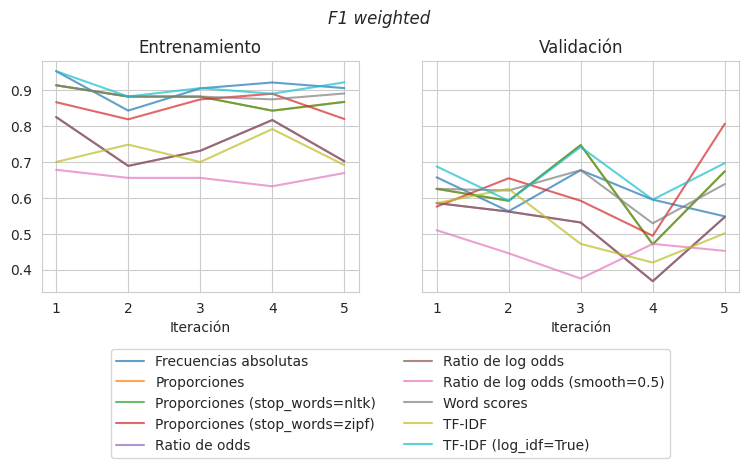
\includegraphics[scale=0.4]{../visualizations/features/f1_weighted_by_split.png}
    \caption{\textit{F1-weighted} o \textit{F1-pesado} por split de validaci\'on
    cruzada para el conjunto de entrenmiento y de testeo, para todos los
    vectorizadores en evaluaci\'on.}
    \label{fig-vectorizers-f1-weighted}
\end{figure}
\FloatBarrier

% cite title
%\usebibentry{monroe2008fightin}{title}

\subsection{Tablas adicionales}\label{appendix-tables}
\subsubsection{Selecci\'on de vectorizador}
\label{appendix-table-vectorizers}

\begin{table}[!htb]
    \centering
    \scalebox{0.8}{
    \begin{tabular}{ |c|c|c|c|c|c|c| }
    \hline
    Vectorizador & Media & Mediana & Desv\'io & M\'aximo \\
    \hline\hline
    Frecuencias absolutas & 0.190 & 0.153 & 0.063 & 0.284 \\
    \hline
    Proporciones & 0.198 & 0.144 & 0.128 & 0.428 \\
    \hline
    Proporciones ($NLTK$) & \cellcolor{highlight-blue!60}0.142 & \cellcolor{highlight-blue!60}0.142 & \cellcolor{highlight-blue!60}0.009 & \cellcolor{highlight-blue!60}0.155 \\
    \hline
    Proporciones ($Zipf$) & 0.249 & 0.170 & 0.147 & 0.449 \\
    \hline
    \textit{Ratio} de \textit{log odds} & 0.184 & 0.148 & 0.088 & 0.341 \\
    \hline
    \textit{Ratio} de \textit{log odds} (suavizado) & 0.286 & 0.258 & 0.141 & 0.470 \\
    \hline
    \textit{Ratio} de \textit{odds} & 0.189 & 0.148 & 0.094 & 0.355 \\
    \hline
    \textit{TF-IDF} & \cellcolor{highlight-orange!60}0.494 & \cellcolor{highlight-orange!60}0.316 & \cellcolor{highlight-orange!60}0.285 & \cellcolor{highlight-orange!60}0.867 \\
    \hline
    \textit{TF-IDF} (\textit{log IDF}) & 0.422 & 0.289 & 0.199 & 0.644 \\
    \hline
    \textit{Word scores} & 0.304 & 0.228 & 0.143 & 0.484 \\
    \hline
\end{tabular}}
\caption{Tiempos de ajuste observados tras vectorizar los discursos analizados
con las distintas t\'ecnicas estad\'isticas y luego entrenar un modelo de
regresi\'on log\'istica \textit{baseline}. Las celdas resaltadas en azul corresponden
a la estategia de vectorizaci\'on que present\'o el mejor tiempo de entrenamiento y las
resaltadas en naranja, a la que obtuvo el peor tiempo.}
\label{table-appendix-fit-time}
\end{table}
%\FloatBarrier



   

\listoftodos%

\end{document}
